\section{PCPP1 Certification}
\subsection{Exam Syllabus}
%
\includepdf[pages=-]{../pdf_pcpp1/pcpp1.pdf}

The exam syllabus can be accessed \href{https://pythoninstitute.org/assets/628def5091da2303121759.pdf}{here}.

\begin{table}[htbp]
    \centering
    \begin{tabular}{lll} % Define the columns with left-aligned, left-aligned, and right-aligned alignment
        \toprule
        \textbf{Section} & \textbf{Items} & \textbf{Max Score} \\
        \midrule
        Section 1: Advanced Object-Oriented Programming & 15 & 42 (35\%) \\
        Section 2: Coding Conventions, Best Practices, and Standarization  & 7 & 14 (12\%) \\
        Section 3: GUI Programming & 8 & 24 (20\%) \\
        Section 4: Network Programming & 8 & 22 (18\%) \\
        Section 5: File Processing and Communicating with a Program’s Environment & 7 & 18 (15\%) \\
        \bottomrule
    \end{tabular}
    \caption{Exam Syllabus}
    \label{tab:exam_sections}
\end{table}

\newpage
\subsection{Exam Questions}

\subsubsection{Shallow Copy vs Deep Copy}
\begin{itemize}
    \item \textbf{copy.copy(original\_list)}: This method creates a shallow copy of \texttt{original\_list}. It means that the top-level elements of the list are copied, but the nested lists are still referenced. Therefore, modifying elements within the nested lists in the copied list will affect the original list as well.
    
    \item \textbf{copy.deepcopy(original\_list)}: This method creates a deep copy of \texttt{original\_list}. It recursively copies all nested lists and objects within \texttt{original\_list}, creating new objects in memory. Therefore, modifying elements within the nested lists in the copied list will not affect the original list.
\end{itemize}

\begin{codebox}
\begin{minted}{python}
# Original list containing strings and a nested list
title = ['Python', 'Course', [3, 10, 0]]

# Shallow copy of the original list
copied = title[:]

# Modify the nested list in the original list
copied[2][1] = 11
copied[0] = "React"

# Print the original list and the shallow copy
print(title)  # Output: ['Python', 'Course', [3, 11, 0]]
print(copied) # Output: ['React', 'Course', [3, 11, 0]]
\end{minted}
\end{codebox}

This operation is known as a \textbf{shallow copy} because it creates a new list object, but it does not create new copies of the elements within the list. If the elements are mutable objects (like lists or dictionaries), changes made to those elements in \texttt{copied} will also be reflected in the original list, and vice versa. However, if the elements are immutable (like integers or strings), they are effectively copied, and changes made to them in one list will not affect the other.

\subsubsection{Copying Comparison}
\begin{codebox}
\begin{minted}{python}
import copy
 
a = [[1, 2], [3, 4]]
 
b = copy.copy(a)
c = copy.deepcopy(a)
 
b[0][0] = 10
c[0][0] = 20

print(a)   # [[10, 2], [3, 4]]
print(b)   # [[10, 2], [3, 4]]
print(c)   # [[20, 2], [3, 4]]
\end{minted}
\end{codebox}

\subsubsection{Copying Performance}
Deep copy will have the worst performance among the provided copy operations. Deep copying, as performed by copy.deepcopy(), creates a new object and recursively copies all nested objects within it. In the case of a large and complex data structure, deep copying can be computationally expensive and time-consuming. It requires traversing the entire structure, creating new objects, and copying the values of all nested objects.

\subsubsection{Copies and id()}
\begin{codebox}
\begin{minted}{python}
title = 'Python Course'
var = title
 
print(f'title ID: {id(title)}') # title ID: 2081709060592
print(f'var ID: {id(var)}')     # var ID: 2081709060592
print(title == var)             # True
print(title is var)             # True
\end{minted}
\end{codebox}

\subsubsection{Deep copy of string}
In the following code example, \texttt{copy.deepcopy()} is used to create a deep copy of the \texttt{title} variable. A deep copy creates a new object and recursively copies the contents of the original object, so changes made to the copied object do not affect the original object, and vice versa.\\

\begin{codebox}
\begin{minted}{python}
import copy

title = 'Python Course'
var = copy.deepcopy(title)
 
print(f'title ID: {id(title)}') # title ID: 2081702974320
print(f'var ID: {id(var)}')     # var ID: 2081702974320
print(title == var)             # True
print(title is var)             # True
\end{minted}
\end{codebox}

However, in this specific case, since the \texttt{title} variable is a string, which is immutable in Python, the deep copy operation does not actually create a new object. Python optimizes memory usage for immutable objects, \textbf{so when a deep copy is made of an immutable object, Python will reuse the existing object rather than creating a new one}.

\subsubsection{Copies}
\begin{codebox}
\begin{minted}{python}
title = ['Python', 'Course', '3.10'] 
copy = title[:]
 
print(f'title ID: {id(title)}') # ...504
print(f'copy ID: {id(copy)}') # ...616
print(title == copy) # True
print(title is copy) # False

print(id(title[0])) # ...040
print(id(copy[0]))  # ...040
\end{minted}
\end{codebox}

\begin{itemize}
\item \texttt{copy = title[:]}: This line creates a shallow copy of the title list and assigns it to the variable copy. The [:] slice notation creates a copy of the entire list.
\item \texttt{print(f'title ID: {id(title)}')}: This line prints the ID of the title list.
\item \texttt{print(f'copy ID: {id(copy)}')}: This line prints the ID of the copy list.
\item \texttt{print(title == copy)}: This line compares the content of the title and var lists. It will return True if the lists have the same elements in the same order, and False otherwise.
\item \texttt{print(title is copy)}: This line checks if title and copy refer to the same object (same ID) in memory. It will return True if title and var are the same object, and False otherwise.
\end{itemize}

\subsubsection{What does the \texttt{id()} function?}
The id() function in Python returns a unique identifier for an object. It is an integer value that represents the "identity" of the object. This identity is guaranteed to be unique and constant for the object during its lifetime, meaning that it will not change as long as the object exists.

\subsubsection{What function determines the type of an object, including functions and classes?}
The \texttt{type()} function is used to determine the type of an object. It can be used with various types of objects, including functions and classes.

\begin{itemize}
    \item \textbf{Type of a Function:} When you use \texttt{type()} with a function, it returns the type of the function object, which is typically \texttt{<class 'function'>}.
    
    \item \textbf{Type of a Class:} When you use \texttt{type()} with a class, it returns the type of the class object, which is typically \texttt{<class 'type'>}.
\end{itemize}

\begin{codebox}
\begin{minted}{python}
def my_func():
    pass

class MyClass:
    pass

print(type(my_func)) # <class 'function'>
print(type(MyClass)) # <class 'type'>
\end{minted}
\end{codebox}

\subsubsection{Logging}
\textbf{In a Python application, you want to customize the format of the log messages. You decide to include the time of logging, the severity level of the message, the module where the event occurred, and the message itself. Which of the following formatting strings would be the most appropriate for this purpose?}\\

\texttt{\%(asctime)s - \%(levelname)s - \%(module)s - \%(message)s}\\

This format string includes the time (\%(asctime)s), the module where the event occurred (\%(module)s), the severity level of the message (\%(levelname)s), and the message itself (\%(message)s).\\

\subsubsection{Which of the following logs represents the default formatting of the root logger in the logging module?}

\texttt{CRITICAL:root:Message}.\\
In the logging module of Python, the default log message format consists of the following components:

\begin{itemize}
    \item \textbf{LEVEL:} Represents the severity level of the log message, such as DEBUG, INFO, WARNING, ERROR, or CRITICAL.
    \item \textbf{LOGGER\_NAME:} The name of the logger used to log the message. The root logger, which is the main logger in the logging hierarchy, is named "root" by default.
    \item \textbf{MESSAGE:} The actual content of the log message.
\end{itemize}

\subsubsection{Logging}
\textbf{The \texttt{logging.basicConfig} function is used to configure the logging module in Python. It allows you to specify the format of log messages using the \texttt{format} argument. The desired log format can be achieved by specifying the appropriate format string with the required attributes of the \texttt{LogRecord} object. What formatting should you apply to get the following?}\\

\texttt{2024-02-08 16:35:27,164 krako WARNING:Your log message}

\begin{codebox}
\begin{minted}{python}
import logging
 
FORMAT = '%(asctime)s %(user)s %(levelname)s:%(message)s'
logging.basicConfig(format=FORMAT)
\end{minted}
\end{codebox}

The \texttt{logging.basicConfig(format=FORMAT)} call sets the format of the root logger to the specified format. This ensures that all subsequent log messages logged through the root logger will use the specified format.
\begin{itemize}
    \item \texttt{\%asctime}: The timestamp of the log entry in the format "YYYY-MM-DD HH:MM:SS,sss".
    \item \texttt{\%user}: The user attribute of the \texttt{LogRecord} object. (Note: This attribute is not available by default, so you may need to add it yourself if it's not present in the \texttt{LogRecord}.)
    \item \texttt{\%levelname}: The log level of the message, e.g., "WARNING" in this case.
    \item \texttt{:} A separator between the log level and the log message.
    \item \texttt{\%message}: The actual log message.
\end{itemize}

\subsubsection{As a Python Developer, you need to work with logging events in your application. Which of the following snippet of code will return the root logger?}
\begin{codebox}
\begin{minted}{python}
import logging
 
logger = logging.getLogger()
\end{minted}
\end{codebox}
In the Python logging module, the \texttt{getLogger()} function is used to retrieve a logger object. By default, if no name is provided as an argument to \texttt{getLogger()}, it returns the root logger.

\newpage
\subsubsection{How can you access the docstring of a function?}

\begin{codebox}
\begin{minted}{python}
def my_function():
    """One-line description."""
    pass

print(my_function.__doc__) # One-line description.
\end{minted}
\end{codebox}

%%%%%%%%%%%%%%%%%%%%%%%%%%%% XML %%%%%%%%%%%%%%%%%%%%%%%%%%

\subsubsection{XML}
\begin{codebox}
\begin{minted}{python}
import xml.etree.ElementTree as ET

# XML string
xml_as_string = '''<?xml version="1.0"?>
<catalog>
   <book id="bk101">
      <author>Gambardella, Matthew</author>
      <title>XML Developer's Guide</title>
      <genre>Computer</genre>
   </book>
   <book id="bk102">
      <author>Ralls, Kim</author>
      <title>Midnight Rain</title>
      <genre>Fantasy</genre>
   </book>
</catalog>'''

# Parse the XML string
root = ET.fromstring(xml_as_string)

# Print tag names and attributes of each element
for child in root:
    print(f'{child.tag} -> {child.attrib}')

# Output
# book -> {'id': 'bk101'}
# book -> {'id': 'bk102'}
\end{minted}
\end{codebox}

\subsubsection{XML Root Element}

In Python's \texttt{xml.etree.ElementTree} module the method \texttt{getroot()} returns the root element of an ElementTree object. Therefore, to obtain the root element of the XML tree represented by the tree object in the provided code, you would use the \texttt{getroot()} method.

\begin{codebox}
\begin{minted}{python}
import xml.etree.ElementTree as ET
tree = ET.parse('products.xml')
root_element = tree.getroot()  # Retrieves the root element of the XML tree
\end{minted}
\end{codebox}

\newpage
\subsubsection{Parsing XML}
\begin{codebox}
\begin{minted}{python}
import xml.etree.ElementTree as ET

# Define the XML string
xml_as_string = """<?xml version="1.0"?>
<catalog>
   <book id="bk101">
      <author>Gambardella, Matthew</author>
      <title>XML Developer's Guide</title>
      <genre>Computer</genre>
      <price>44.95</price>
   </book>
   <book id="bk102">
      <author>Ralls, Kim</author>
      <title>Midnight Rain</title>
      <genre>Fantasy</genre>
      <price>5.95</price>
   </book>
</catalog>"""

# Parse the XML string
root = ET.fromstring(xml_as_string)
print(root[0])           # <Element 'book' at 0x000002C183BEF290>
print(root[0][0])        # <Element 'author' at 0x000002C183BEFC90>
print(root[0][0].text)   # Gambardella, Matthew
print(root[1][3].text)   # 5.95
\end{minted}
\end{codebox}

\subsubsection{XPath}
XPath is a query language for selecting nodes from an XML document. When using XPath, the \texttt{@name} syntax is used to select attributes with the specified name. Here's how it works:
\begin{codebox}
\begin{minted}{text}
<bookstore>
  <book name="Harry Potter">
    <author>J.K. Rowling</author>
    <price>20</price>
  </book>
  <book name="The Hobbit">
    <author>J.R.R. Tolkien</author>
    <price>25</price>
  </book>
</bookstore>
\end{minted}
\end{codebox}
If you want to select nodes based on the value of an attribute named "name", you would use the \texttt{[@name]} syntax in your XPath expression. This will select nodes that have a "name" attribute, regardless of its value. 
\begin{itemize}
\item If you want to select all \texttt{<book>} elements that have a "name" attribute, you would use the XPath expression: \textbf{\texttt{//book[@name]}}
\item To find all books named "The Hobbit" in the XML document, you can use the following XPath expression: \textbf{\texttt{//book[@name='The Hobbit']}}
\end{itemize}

\subsubsection{XPath indices}
\textbf{XPath indices start at 1, not 0.} When using XPath to navigate XML documents or select nodes, you start counting from 1 for the first node, 2 for the second node, and so on. This is consistent with many other programming languages and standards where indexing typically starts at 1 instead of 0.\\

\texttt{/store/book[2]/author}: This XPath expression correctly selects the author of the \textbf{second} book in the store.

\subsubsection{Document Type Definition (DTD)}
\textbf{Consider the following Document Type Definition (DTD) for an XML document:}
\begin{minted}{text}
<!DOCTYPE bookstore [
  <!ELEMENT bookstore (book*)>
  <!ELEMENT book (title, author, year, price)>
  <!ATTLIST book category CDATA #REQUIRED>
  <!ELEMENT title (#PCDATA)>
  <!ELEMENT author (#PCDATA)>
  <!ELEMENT year (#PCDATA)>
  <!ELEMENT price (#PCDATA)>
]>
\end{minted}

\begin{itemize}
\item \textbf{The "book" element must contain the child elements in the order of "title", "author", "year", and "price".} According to the DTD, the "book" element must contain the child elements in the specified order: "title", "author", "year", and "price".

\item \textbf{The "book" element must have an attribute called "category" of type CDATA.} The DTD specifies that the "book" element must have an attribute called "category" with a type of CDATA. The \texttt{\#REQUIRED} keyword indicates that the attribute is mandatory.

\item \textbf{\texttt{\#PCDATA}} stands for "Parsed Character Data." It is a keyword used to specify that an element can contain character data that will be parsed by the XML parser.\\

\item \textbf{\texttt{!ELEMENT}} is used to define the structure of elements (their names and content models), while \texttt{!ATTLIST} is used to define the attributes of elements (their names, datatypes, and properties).
\end{itemize}

\subsubsection{XML Attributes}
\begin{codebox}
\begin{minted}{xml}
<person id="123" gender="female">
    <name>Emma</name>
    <age>30</age>
</person>
\end{minted}
\end{codebox}

In this code example, \texttt{id} and \texttt{gender} are attributes of the \texttt{<person>} element.

\subsubsection{XML - Comments}
In XML (eXtensible Markup Language), comments are used to add explanatory or informative text that is not processed by the XML parser. An XML comment is a text surrounded by \texttt{<!-- and !-->}.

\newpage
\subsubsection{Write XML}
You can use the \texttt{xml.etree.ElementTree} module in Python to create the XML file. This code will create an XML file named "books.xml" with the specified structure and content.
\begin{codebox}
\begin{minted}{python}
import xml.etree.ElementTree as ET

# Create the root element
catalog = ET.Element("catalog")

# Create the first book element
book1 = ET.SubElement(catalog, "book", id="bk101")
book1.text = ""
ET.SubElement(book1, "author").text = "Gambardella, Matthew"
ET.SubElement(book1, "title").text = "XML Developer's Guide"
ET.SubElement(book1, "genre").text = "Computer"
ET.SubElement(book1, "price").text = "44.95"
ET.SubElement(book1, "publish_date").text = "2000-10-01"

# Create the second book element
book2 = ET.SubElement(catalog, "book", id="bk102")
book2.text = ""
ET.SubElement(book2, "author").text = "Ralls, Kim"
ET.SubElement(book2, "title").text = "Midnight Rain"
ET.SubElement(book2, "genre").text = "Fantasy"
ET.SubElement(book2, "price").text = "5.95"
ET.SubElement(book2, "publish_date").text = "2000-12-16"

# Create the XML tree
tree = ET.ElementTree(catalog)

# Write the XML tree to a file
tree.write("books.xml", encoding="utf-8", xml_declaration=True)
\end{minted}
\end{codebox}

\textbf{books.xml:}
\begin{minted}{xml}
<?xml version='1.0' encoding='utf-8'?>
<catalog>
	<book id="bk101">
		<author>Gambardella, Matthew</author>
		<title>XML Developer's Guide</title>
		<genre>Computer</genre>
		<price>44.95</price>
		<publish_date>2000-10-01</publish_date>
	</book>
	<book id="bk102">
		<author>Ralls, Kim</author>
		<title>Midnight Rain</title>
		<genre>Fantasy</genre>
		<price>5.95</price>
		<publish_date>2000-12-16</publish_date>
	</book>
</catalog>
\end{minted}

\subsubsection{Parsing XML}
\textbf{How can you parse the document "books.xml" document using xml.etree.ElementTree module?}

\begin{codebox}
\begin{minted}{python}
import xml.etree.ElementTree as ET

# Parse the XML file and create a tree
tree = ET.parse('books.xml')

# Get the root element of the tree
root = tree.getroot()  

# Convert the root element to a string
tree_str = ET.tostring(root)
\end{minted}
\end{codebox}
This code snippet correctly imports the \texttt{xml.etree.ElementTree} module and then uses the \texttt{ET.parse()} function to read and parse the XML document named "books.xml". The resulting parsed tree object is stored in the tree variable, which can be further manipulated or accessed to extract information from the XML document.

\subsubsection{Create an XML file}
As a Python Developer, you need to create an XML file with the following structure using Python:

\begin{minted}{text}
<movies>
  <movie>
    <title>The Shawshank Redemption</title>
    <rate>9.2</rate>
  </movie>
</movies>
\end{minted}

\textbf{Which of the following snippet of code should you use?}
\begin{codebox}
\begin{minted}{python}
import xml.etree.ElementTree as ET

root = ET.Element('movies') # Must be ET.Element

movie1 = ET.SubElement(root, 'movie') # Must be ET.SubElement
ET.SubElement(movie1, 'title').text = 'The Shawshank Redemption'
ET.SubElement(movie1, 'rate').text = '9.2'

tree = ET.ElementTree(root)
tree.write('movies.xml') # Must be tree.write()
\end{minted}
\end{codebox}

\subsubsection{Writing CSV files}
\textbf{As a Python Developer, you need to save data to a CSV file named "items.csv", and you want the file structure as follows:}

\begin{minted}{text}
name,quantity
laptop,3
mobile phone,2
car,1
\end{minted}

\textbf{Which of the following code snippets will do this job? }

\begin{itemize}
\item This code snippet correctly saves data to the 'items.csv' file with the desired structure. It uses the \texttt{csv} module to handle CSV operations. The \texttt{DictWriter} class is used to write rows based on dictionaries, and the \texttt{writeheader()} method is used to write the header row. The data rows are then written using \texttt{writerow()} with dictionaries representing the name and quantity values.
\begin{codebox}
\begin{minted}{python}
import csv
 
with open('items.csv', 'w', newline='') as csvfile:
    fieldnames = ['name', 'quantity']
    writer = csv.DictWriter(csvfile, fieldnames=fieldnames)
    writer.writeheader()
    writer.writerow({'name': 'laptop', 'quantity': 3})
    writer.writerow({'name': 'mobile phone', 'quantity': 2})
    writer.writerow({'name': 'car', 'quantity': 1})
\end{minted}
\end{codebox}
\item This code snippet also correctly saves data to the 'items.csv' file with the desired structure. It uses the \texttt{csv} module and the \texttt{writer()} function to create a writer object for writing rows. The header row and data rows are written using \texttt{writerow()} with lists representing the name and quantity values.
\begin{codebox}
\begin{minted}{python}
import csv
 
with open('items.csv', 'w', newline='') as csvfile:
    writer = csv.writer(csvfile)
    writer.writerow(['name', 'quantity'])
    writer.writerow(['laptop', 3])
    writer.writerow(['mobile phone', 2])
    writer.writerow(['car', 1])
\end{minted}
\end{codebox}
\end{itemize}


%%%%%%%%%%%%%%%%%%%%%%%%%% PEP %%%%%%%%%%%%%%%%%%%%%%%%%%
\subsubsection{Which naming style does PEP 8 recommend for package names?}
A lower-case word or words that are not separated, e.g. \textbf{mypackagename}. PEP 8 is a style guide for Python code, and it provides recommendations on how to format Python code for maximum readability and consistency. In the case of package names, PEP 8 recommends using a lower-case word or words that are \textbf{not separated}.

\subsubsection{PEP 8 - Docstrings}
One-line docstrings are typically used for simple functions or methods, while multi-line docstrings are typically used for more complex functions or methods, or classes. A one-line docstring is a brief summary of what a function, method, or class does. A multi-line docstring typically starts with a one-line summary followed by a more detailed explanation, if necessary. The latter is often used for complex functions, methods, or classes that need a more detailed explanation. It may also contain additional sections like parameters, return values, and exceptions raised.

\newpage
\subsubsection{Which of the following statements regarding PEP 8 guidelines and documentation strings for the given code snippet is correct?}
\begin{codebox}
\begin{minted}{python}
def calculate_discounted_price(original_price, discount):
    """
    Calculates the discounted price based on the original price and discount.
 
    Parameters:
    - original_price (float): The original price of the item.
    - discount (float): The discount percentage to be applied.
 
    Returns:
    - discounted_price (float): The calculated discounted price.
 
    Example:
    >>> calculate_discounted_price(100, 20)
    80.0
    """
    discounted_price = original_price * (1 - discount/100)
    return discounted_price
\end{minted}
\end{codebox}

The function definition adheres to the PEP 8 guidelines as it uses meaningful variable names and includes a detailed documentation string.  The code follows the naming conventions and includes a well-documented docstring that provides information about the function's purpose, parameters, return value, and an example usage.\\

For consistency, you should always use \textbf{triple double quotes} around docstrings. PEP 258, which provides guidelines for documenting Python programs, recommends using \texttt{"""} triple double quotes \texttt{"""} around docstrings for consistency. While single quotes or triple single quotes can also be used, it is generally recommended to use triple double quotes to maintain consistency throughout the codebase.

\subsubsection{Which of the following code snippets follow the PEP 8 recommendation for blank lines?}
PEP 8 recommends that you should use two blank lines to surround top-level function and class definitions.

\begin{codebox}
\begin{minted}{python}
class Container:
    pass
 

class PlasticContainer(Container):
    pass
 

class MetalContainer(Container):
    pass
\end{minted}
\end{codebox}

\newpage
\subsubsection{What is the order of imports recommended by PEP 8?}
PEP 8 suggests a specific order to import different types of modules:
\begin{enumerate}
    \item Standard library imports
    \item Related third-party imports
    \item Local application/library-specific imports
\end{enumerate}

\subsubsection{PEP 8 - Docstrings}
\begin{itemize}
\item The docstring for a module should generally list the classes, exceptions and functions that are exported by the module, with a one-line summary of each. The docstring for a module is typically used to provide an overview of the module's purpose and functionality, including a summary of the classes, exceptions, and functions that are part of the module.

\item The docstring for a function or method should summarize its behavior and document its arguments, return value(s), side effects, exceptions raised, and restrictions on when it can be called (all if applicable). The docstring for a function or method should provide a concise summary of its purpose and describe important details such as the expected arguments, return values, any side effects, exceptions that can be raised, and any restrictions or conditions for calling the function or method.

\item The purpose of the class docstring is to summarize the behavior and purpose of the class as a whole, rather than providing a detailed listing of its methods and attributes.

\item There is no requirement for two blank lines after the summary line. The use of two blank lines is a convention, but it is not strictly mandated by PEP 257.
\end{itemize}

\subsubsection{PEP - Quotes}
In Python, single-quoted strings and double-quoted strings are the same. This PEP does not make a recommendation for this. Pick a rule and stick to it. When a string contains single or double quote characters, however, \textbf{use the other one to avoid backslashes} in the string. It improves readability.

\begin{codebox}
\begin{minted}{python}
# Consistent use of single quotes
string1 = 'This is a string with "double quotes" inside.'

# Consistent use of double quotes
string2 = "This is a string with 'single quotes' inside."
\end{minted}
\end{codebox}

\subsubsection{Block comments in Python according to PEP...}
\begin{itemize}
\item \textbf{should refer to the code that follows them.} Block comments are used to provide explanatory information about the code that follows them. They help document and clarify the purpose or functionality of the code. By placing the comments before the relevant code, they provide context and aid in understanding the code's intent or behavior.

\item \textbf{should be indented to the same level as the code they describe.} According to PEP 8, block comments should be indented to the same level as the code they describe. This maintains code readability and ensures that the comments are visually associated with the code they are explaining. Consistent indentation helps to clearly identify the relationship between comments and the corresponding code.

\end{itemize}

\subsubsection{PEP 8 recommendations for using whitespace}

\begin{itemize}
\item Immediately inside parentheses, brackets or braces:
\begin{codebox}
\begin{minted}{python}
# Correct:
spam(ham[1], {eggs: 2})

# Wrong:
spam( ham[ 1 ], { eggs: 2 } )
\end{minted}
\end{codebox}

\item Immediately before the open parenthesis that starts an indexing or slicing:
\begin{codebox}
\begin{minted}{python}
# Correct:
dct['key'] = lst[index]

# Wrong:
dct ['key'] = lst [index]
\end{minted}
\end{codebox}

\item More than one space around an assignment operator to align it with another:
\begin{codebox}
\begin{minted}{python}
# Correct:
x = 1
y = 2
long_variable = 3

# Wrong:
x             = 1
y             = 2
long_variable = 3
\end{minted}
\end{codebox}
\end{itemize}


%%%%%%%%%%%%%%%%%%%%%%%%%%% DATABASES %%%%%%%%%%%%%%%%%%%%%%%%%%
\newpage
\subsubsection{Features of SQLite databases}

\begin{itemize}
\item \textbf{Serverless:} \textbf{(True)} SQLite databases are serverless, meaning they don't require a separate server process to operate. The entire database is stored as a single disk file, making it easy to manage and deploy without the need for a dedicated database server.

\item \textbf{Zero-Configuration:} \textbf{(True)} SQLite databases are known for their zero-configuration nature. You don't need to set up a separate server or configure complex settings to start using SQLite. It's designed to work out of the box with minimal setup requirements.

\item \textbf{Transactional:} \textbf{(True)} SQLite databases support transactions, which ensure that a series of database operations either all succeed or all fail together. This ACID (Atomicity, Consistency, Isolation, Durability) property ensures data integrity and reliability, making SQLite suitable for applications that require transactional support.

\item \textbf{Highly Scalable:} \textbf{(False)} SQLite databases are not as scalable as some other database systems like PostgreSQL or MySQL. While they can handle moderate workloads and data sizes efficiently, they may not be suitable for very large-scale applications or high-concurrency scenarios. However, SQLite databases can still be scaled horizontally by distributing multiple database files across different storage devices.
\end{itemize}

\begin{itemize}[label=--]
    \item Transactions are atomic, consistent, isolated, and durable (ACID) even after system crashes and power failures.
    \item Zero-configuration - no setup or administration needed.
    \item Full-featured SQL implementation.
    \item A complete database is stored in a single cross-platform disk file.
    \item Supports terabyte-sized databases and gigabyte-sized strings and blobs.
    \item Small code footprint: less than 750KiB fully configured or much less with optional features omitted.
    \item Simple, easy to use API.
    \item Fast: In some cases, SQLite is faster than direct filesystem I/O.
    \item Written in ANSI-C. TCL bindings included. Bindings for dozens of other languages available separately.
    \item Well-commented source code with 100\% branch test coverage.
    \item Available as a single ANSI-C source-code file that is easy to compile and hence is easy to add into a larger project.
    \item Self-contained: no external dependencies.
    \item Cross-platform: Android, *BSD, iOS, Linux, Mac, Solaris, VxWorks, and Windows (Win32, WinCE, WinRT) are supported out of the box. Easy to port to other systems.
    \item Sources are in the public domain. Use for any purpose.
    \item Comes with a standalone command-line interface (CLI) client that can be used to administer SQLite databases.
\end{itemize}

\newpage
\subsubsection{SQLite in memory}
To connect to a SQLite database in memory (RAM) using Python, you can use the sqlite3 module, which comes pre-installed with Python. You can establish a connection to an in-memory SQLite database by specifying the special filename ":memory:". Here's the code to connect to an SQLite in-memory database:
\begin{codebox}
\begin{minted}{python}
import sqlite3

# Connect to the SQLite in-memory database
connection = sqlite3.connect(":memory:")
\end{minted}
\end{codebox}

\subsubsection{Create a table}
In Python, using the sqlite3 module, how would you create a table named Students in a SQLite database that has columns for ID (an integer), Name (a text), Major (a text), and Year (an integer)? Assume the database connection is already established and stored in the variable conn.
\begin{codebox}
\begin{minted}{python}
import sqlite3

# Establish a connection to the SQLite database
conn = sqlite3.connect(":memory:")

# Create a cursor object to execute SQL commands
cursor = conn.cursor()

# SQL statement to create the Students table
create_table_query = """
CREATE TABLE IF NOT EXISTS Students (
    ID INTEGER PRIMARY KEY,
    Name TEXT,
    Major TEXT,
    Year INTEGER
);
"""
\end{minted}
\end{codebox}

\subsubsection{SQLite - SELECT}
\textbf{Consider a SQLite database with a table named Employees that has the columns EmployeeID, FirstName, LastName, HireDate. Which of the following commands correctly retrieves all records of employees who were hired after January 1, 2023?}\\

\texttt{SELECT * FROM Employees WHERE HireDate > '2023-01-01';}\\ This is the correct syntax to retrieve all records where the HireDate is after January 1, 2023. The SELECT keyword is used to specify the columns to be returned (in this case, all columns), the FROM keyword specifies the table, and the WHERE keyword specifies the condition.

\newpage
\subsubsection{Sqlite3}
\begin{codebox}
\begin{minted}{python}
import sqlite3

# Connect to the SQLite database named 'company.db'
conn = sqlite3.connect('company.db')

# Create a cursor object to execute SQL commands
c = conn.cursor()

# Execute an SQL command to create a table named 'Employees'
# The table has four columns: ID, NAME, ADDRESS, and SALARY
c.execute('''
    CREATE TABLE Employees (
        ID INT PRIMARY KEY NOT NULL,
        NAME TEXT NOT NULL,
        ADDRESS CHAR(50),
        SALARY REAL
    );
''')

# Commit the changes and close the connection
conn.commit()
conn.close()
\end{minted}
\end{codebox}
\begin{itemize}
    \item After creating the table, use braces to enclose the list of fields.
    \item Include a comma after every new field definition within the braces.
    \item End the entire SQL command with a semicolon to denote the end of the statement.
\end{itemize}

\subsubsection{Sqlite3}
To save changes made to an SQLite database, you need to ensure that you commit the changes before closing the connection.
\begin{codebox}
\begin{minted}{python}
import sqlite3

# Connect to the database
conn = sqlite3.connect('employee.db')
c = conn.cursor()

# Execute SQL code to insert data
sql_code = """INSERT INTO Employees 
VALUES (1, 'John Doe', 30, 50000)"""
c.execute(sql_code)

# Commit changes to the database
conn.commit()

# Close the connection
conn.close()
\end{minted}
\end{codebox}

\newpage
\subsubsection{SQLite database - Creating a table}
\textbf{You need to create a table named Products in an SQLite database using the sqlite3 module in Python. The table should have the following columns:}

\begin{itemize}
    \item \textbf{ProductID}: A unique identifier for each product, represented as an INTEGER and serving as the primary key.
    \item \textbf{Name}: The name of the product, stored as TEXT.
    \item \textbf{Price}: The price of the product, stored as REAL.
    \item \textbf{CategoryID}: An identifier linking each product to its category, represented as an INTEGER and serving as a foreign key to the "Categories" table.
\end{itemize}

\begin{codebox}
\begin{minted}{python}
import sqlite3

# Connect to the SQLite database (or create it if it doesn't exist)
conn = sqlite3.connect('products.db')

# Create a cursor object to execute SQL queries
cursor = conn.cursor()

# Create the Products table
cursor.execute('''CREATE TABLE IF NOT EXISTS Products (
                    ProductID INTEGER PRIMARY KEY,
                    Name TEXT,
                    Price REAL,
                    CategoryID INTEGER,
                    FOREIGN KEY (CategoryID) REFERENCES Categories(CategoryID)
                )''')

# Commit the changes and close the connection
conn.commit()
conn.close()
\end{minted}
\end{codebox}

\subsubsection{Connect to SQLite database}
\textbf{As a Python Developer, you want to connect to a SQLite database named "app.db". Which code will you use?}

\begin{codebox}
\begin{minted}{python}
import sqlite3
 
conn = sqlite3.connect('app.db')
\end{minted}
\end{codebox}

To connect to a SQLite database in Python, you need to import the sqlite3 module and use the \texttt{connect()} function. The \texttt{connect()} function takes the database file name or path as an argument.

\subsubsection{SQLite database operations}
\begin{itemize}
    \item \texttt{executemany()}: Insert multiple rows of data into a table.
    
    \item \texttt{fetchone()}: Retrieve the next row of a query result set.
    
    \item \texttt{execute()}: Run a single SQL query.
    
    \item \texttt{fetchall()}: Fetch all rows of a query result set.
\end{itemize}

\newpage
\subsubsection{In-memory SQLite database}
\begin{codebox}
\begin{minted}{python}
import sqlite3
from sqlite3 import Error
 
def create_connection():
    conn = None;
    try:
        conn = sqlite3.connect(':memory:')       
        print(sqlite3.version)
    except Error as e:
        print(e)
    finally:
        if conn:
            conn.close()
 
if __name__ == '__main__':
    create_connection()
\end{minted}
\end{codebox}

The code \textbf{\texttt{conn = sqlite3.connect(':memory:')}} will create a new, temporary, in-memory SQLite database. This database exists only for the duration of the connection and resides entirely in memory. Once the connection is closed with \texttt{conn.close()}, the database is destroyed, and all its contents are lost.

\subsubsection{SQLite}
A table with the following structure (SQLite) is given:

\begin{codebox}
\begin{minted}{python}
CREATE TABLE users (
    first_name TEXT,
    last_name TEXT,
    email TEXT
);
\end{minted}
\end{codebox}

\textbf{Which statements will insert a record into this table?}

\begin{itemize}
\item This statement correctly inserts a record into the users table by specifying the column names in the INSERT INTO statement and providing the corresponding values in the VALUES clause. The values 'Mike', 'Smith', and 'mike.smith@esmartdata.org' are inserted into the columns first\_name, last\_name, and email, respectively.
\begin{codebox}
\begin{minted}{python}
INSERT INTO users (first_name, last_name, email)
VALUES ('Mike', 'Smith', 'mike.smith@esmartdata.org');
\end{minted}
\end{codebox}

\item This statement also correctly inserts a record into the users table. In this case, the INSERT INTO statement omits the column names and directly provides the values in the order they are defined in the table structure. The values 'Mike', 'Smith', and 'mike.smith@esmartdata.org' are inserted into the respective columns in the order they appear in the table.
\begin{codebox}
\begin{minted}{python}
INSERT INTO users VALUES ('Mike', 'Smith', 'mike.smith@esmartdata.org');
\end{minted}
\end{codebox}
\end{itemize}

%%%%%%%%%%%%%%%%%%%%%%%%%%% NETWORKING %%%%%%%%%%%%%%%%%%%%%%%%%%
\newpage
\subsubsection{Sockets - \texttt{accept()}}

The method of the socket module that allows a server socket to accept requests from a client socket from another host is accept(). When a server socket is listening for connections, it can call the accept() method to accept an incoming connection request from a client socket. This method blocks until a connection is established or a timeout occurs.

\begin{codebox}
\begin{minted}{python}
import socket

server_socket = socket.socket(socket.AF_INET, socket.SOCK_STREAM)
# Bind to all available interfaces on port 8888
server_socket.bind(('0.0.0.0', 8888))
# Listen for incoming connections, allow up to 1 connection in the backlog
server_socket.listen(1)

print("Server is listening for incoming connections...")
# Accept an incoming connection
client_socket, client_address = server_socket.accept()

print(f"Connection established with {client_address}")
\end{minted}
\end{codebox}

\subsubsection{Sockets - \texttt{recv()}}
\textbf{You are implementing a client-server communication program in Python using sockets. The server sends a large amount of data to the client in chunks. The client uses the recv() method to receive the data. Which statement about the recv() method is correct in this scenario?}
\begin{itemize}
\item The recv() method may return less data than requested, even if more data is available on the server. The recv() method does not guarantee that it will return all the data in one call. It may return a smaller chunk of data, and you need to handle multiple calls to recv() to receive the complete data.
\item The recv() method will block until it receives all the data sent by the server or until an error occurs. The recv() method will block until it receives at least one byte of data or until a timeout or error occurs. It does not guarantee that it will receive all the data in one call.
\end{itemize}

\subsubsection{Which method of the socket module allows you to send data to a given address?}
The \texttt{socket.sendto(data, address)} method is used to send data to a specific address using a socket. It takes two parameters: data, which is the data to be sent as a bytes-like object, and address, which is the destination address to send the data to.

By calling the \texttt{sendto()} method on a socket object, you can send data to the specified address. This method is typically used with UDP (User Datagram Protocol) sockets, where data is sent as individual packets without establishing a persistent connection.


\subsubsection{API requires authentication}
\textbf{You are developing a Python application that needs to communicate with a web API to retrieve data. The API requires authentication using an API key. Which of the following HTTP header fields should be used to include the API key in the request?}\\

The "Authorization" header field should be used to include the API key in the request. It is commonly used for providing authentication credentials, including API keys, in HTTP requests.

\subsubsection{Asynchronous I/O}
\textbf{You are developing a Python application that requires efficient and scalable network communication for handling a large number of concurrent connections. Which of the following network programming paradigms or frameworks would be most suitable for achieving this requirement?}

Asynchronous I/O (asyncio) is a programming paradigm in Python that enables efficient and scalable network communication. It allows handling a large number of concurrent connections with a single thread by utilizing non-blocking I/O operations and coroutines. asyncio provides built-in support for writing high-performance networking code.

\subsubsection{How can you access the headers and content-type information?}
Suppose you have the following request:
\begin{codebox}
\begin{minted}{python}
import requests
 
reply = requests.get('http://python.org:80')
\end{minted}
\end{codebox}

\textbf{\texttt{reply.headers['Content-Type']}}\\
In the given code snippet, the requests.get() function is used to send an HTTP GET request to the URL 'http://python.org:80'. The response from the server is stored in the reply variable. To access the headers and content-type information of the response, you can use the headers attribute of the response object, followed by the specific header field you want to retrieve. This option correctly accesses the value of the 'Content-Type' header field in the response. The headers attribute returns a dictionary-like object, and you can use square brackets [] with the desired header field name as the key to access its value. In this case, we want to retrieve the value of the "Content-Type" header, which indicates the MIME type of the content in the response.\\

\textbf{Server’s response headers example:}

\begin{minted}{text}
{
    'Connection': 'keep-alive',
    'Content-Length': '49892',
    'Server': 'nginx',
    'Content-Type': 'text/html; charset=utf-8',
    'X-Frame-Options': 'DENY',
    'Via': '1.1 vegur, 1.1 varnish',
    'Accept-Ranges': 'bytes',
    'Date': 'Wed, 21 Sep 2022 09:26:53 GMT',
    'Age': '1759',
    'X-Served-By': 'cache-iad-kiad7000038-IAD',
    'X-Cache': 'HIT',
    'X-Cache-Hits': '2',
    'X-Timer': 'S1663752414.714920,VS0,VE0',
    'Vary': 'Cookie',
    'Strict-Transport-Security': 'max-age=63072000; includeSubDomains',
}
\end{minted}

\newpage
\textbf{You are developing a Python application that interacts with a RESTful API. As part of the application's functionality, you need to analyze the server's response headers. Which of the following HTTP headers is commonly used to specify the format of the data being returned in the response?}

\begin{itemize}
    \item \textbf{Content-Type} $\rightarrow$ Correct. This header is commonly used to indicate the media type or content type of the response. It specifies the format of the data being returned, such as "application/json" or "text/html". This header is directly relevant to determining the content type of the response. Therefore, this is the correct answer.
    \item \textbf{Content-Disposition} $\rightarrow$ Incorrect. This header is used to suggest a filename to the user-agent when the response content is being downloaded. It does not indicate the content type. Therefore, this answer is incorrect.
    \item \textbf{Content-Encoding} $\rightarrow$ Incorrect. This header is used to specify the encoding applied to the response content, such as gzip or deflate. It does not convey information about the content type. Thus, this answer is incorrect.
    \item \textbf{Content-Range} $\rightarrow$ Incorrect. This header is used to indicate the range of bytes being returned in a partial response. It does not provide information about the content type. Thus, this answer is incorrect.
    \item \textbf{Content-Length} $\rightarrow$ Incorrect. This header specifies the size of the response content in bytes. It does not provide information about the content type. Hence, this answer is incorrect.
\end{itemize}

\subsubsection{Protocols}

\begin{itemize}
    \item \textbf{SSL/TLS (Secure Sockets Layer/Transport Layer Security)} is the appropriate protocol for establishing secure encrypted connections between a client and a server. It ensures confidentiality, integrity, and authentication of the transmitted data.
    
    \item \textbf{HTTP (Hypertext Transfer Protocol)} is a protocol used for transferring data over the web but does not inherently provide secure encrypted connections. It operates on top of TCP/IP.
    
    \item \textbf{FTP (File Transfer Protocol)} is primarily used for file transfer and does not offer built-in security features for establishing secure encrypted connections. It operates on top of TCP/IP.
    
    \item \textbf{UDP (User Datagram Protocol)} is a connectionless protocol that does not provide built-in mechanisms for secure encrypted connections. It is used for transmitting data in a fast and efficient manner but does not guarantee delivery or order of arrival.
    
    \item \textbf{TCP (Transmission Control Protocol)} is a connection-oriented protocol that ensures reliable and ordered delivery of data between two devices over a network. While it does not inherently provide encryption, it forms the basis for secure communication protocols like SSL/TLS. TCP is widely used for applications such as web browsing, email, and file transfer.
    
    \item \textbf{IP (Internet Protocol)} is a fundamental protocol in the Internet protocol suite. It is responsible for addressing and routing packets of data so that they can travel across networks and arrive at the correct destination. IP provides the basic framework for delivering data packets from source to destination.
\end{itemize}

\newpage
\subsubsection{Multi-threaded Python application}
\textbf{You are developing a multi-threaded Python application that involves network communication using sockets. Each thread performs socket operations independently. You want to handle exceptions raised during socket operations in a thread-safe manner. Which approach would you use to achieve this?}\\

Create a separate thread for exception handling and use inter-thread communication mechanisms to pass exceptions to it. This approach allows for centralized exception handling while maintaining thread-safety. A dedicated thread can handle exceptions, and inter-thread communication mechanisms such as queues can be used to pass exceptions from worker threads to the exception handling thread.

\subsubsection{Internet Protocol}
\textbf{The IP (Internet Protocol) is one of the lowest parts of TCP/IP protocol stack. It's able to send a packet of data (a datagram) between two network nodes. IP is a very unreliable protocol and it... }
\begin{itemize}
\item \textbf{doesn't guarantee that any of the sent datagrams will reach the target.} This is true because IP is a best-effort delivery protocol, meaning it does not provide any guarantee of delivery. Packets can be lost, dropped, or discarded due to various network conditions, congestion, or failures.
\item \textbf{doesn't guarantee that the datagram will reach the target intact.} This is true because IP does not provide any mechanisms for ensuring the integrity of the data during transmission. Packets can be corrupted or modified during transit, and IP does not have built-in mechanisms for detecting or correcting such errors.
\item \textbf{doesn't guarantee that a pair of sent datagrams will reach the target in the same order as they were sent.} This is true because IP treats each datagram as an independent unit and does not enforce any ordering of packets. Packets can take different paths through the network, and they may arrive at the destination out of order.
\end{itemize}

Internet Protocol is a connectionless protocol. Connection-oriented protocols, such as TCP (Transmission Control Protocol), establish a reliable and ordered connection between two network nodes, whereas IP operates at a lower level and does not establish a connection or provide reliable and ordered delivery.

\subsubsection{Transport Layer Security (TLS)}
\textbf{You are developing a RESTful API for an e-commerce platform. The API needs to handle secure payment transactions. Which of the following network programming concepts is most relevant to ensure the security of payment transactions in the API?}

Transport Layer Security (TLS) is the most relevant network programming concept for ensuring the security of payment transactions in a RESTful API. TLS provides secure communication over a network by encrypting data sent between the client and server, thereby protecting sensitive information, such as payment details, from unauthorized access.

\subsubsection{What is the difference between the TCP and UDP protocols?}
TCP is connection-oriented, while UDP is not.

\newpage
\subsubsection{UDP}
\begin{itemize}
\item UDP uses a simple connectionless communication model. UDP (User Datagram Protocol) is a connectionless transport protocol. It does not establish a persistent connection between the sender and receiver. Each datagram (packet) is sent independently and can take different paths through the network. UDP is often used for applications where real-time or low-latency communication is required.

\item UDP has no handshaking dialogues. Unlike TCP (Transmission Control Protocol), UDP does not involve handshaking dialogues for connection establishment or termination. UDP does not guarantee reliability, ordering, or congestion control. It provides a lightweight, low-overhead communication mechanism without the overhead of establishing and maintaining a connection.

\item The speed of data transmission depends on various factors such as network conditions, data size, and application design. UDP can be faster than TCP in situations where reliability and ordered delivery are not critical, as it has less overhead due to the lack of connection establishment and error recovery mechanisms.

\item UDP is a connectionless protocol and does not establish a connection between the client and server before data can be sent. It does not have a concept of a connection or maintain state information between the communicating parties.
\end{itemize}

\subsubsection{UDP sockets}
\begin{codebox}
\begin{minted}{python}
import socket

udp_socket = socket.socket(socket.AF_INET, socket.SOCK_DGRAM)

udp_socket.bind(('127.0.0.1', 12345))

data, address = udp_socket.recvfrom(1024)
print("Received data:", data.decode())

response = "Message received!"
udp_socket.sendto(response.encode(), address)

udp_socket.close()
\end{minted}
\end{codebox}
\begin{itemize}
\item \texttt{SOCK\_DGRAM}: Create a UDP socket
\item \texttt{sendto()}: Method, which is used for sending data over UDP
\end{itemize}

\newpage
\subsubsection{TCP}
The TCP (Transmission Control Protocol) is one of the core protocols in the TCP/IP protocol stack, which is used for communication over the internet.
\begin{itemize}
\item \textbf{TCP is the highest part of the TCP/IP protocol stack.} The TCP (Transmission Control Protocol) is one of the core protocols in the TCP/IP protocol stack, which is used for communication over the internet. It operates at the transport layer, which is above the network layer and below the application layer. Therefore, it is correct to say that TCP is the highest part of the TCP/IP protocol stack.

\item \textbf{TCP uses segments (provided by the lower layers) and handshakes (an automated process of synchronizing the flow of data) to construct a reliable communication channel able to transmit and receive single characters.} TCP uses segments provided by the lower layers, such as IP (Internet Protocol). It also employs a three-way handshake process to establish a reliable communication channel. This handshake involves a series of messages exchanged between the sender and receiver to synchronize the flow of data. TCP ensures that the data is transmitted and received reliably, not limited to single characters. Therefore, this statement accurately describes how TCP operates.

\item \textbf{TCP guarantees that a stream of data reaches the target, or the sender is informed that communication has failed.} TCP is designed to provide reliable, connection-oriented communication. It guarantees that a stream of data sent by the sender reaches the intended recipient. If any issues or failures occur during the communication process, TCP detects and handles them by retransmitting lost segments, ensuring data integrity and delivery. If the communication fails despite attempts to recover, the sender is informed of the failure.
\end{itemize}

\subsubsection{TCP sockets}
\textbf{Which of the following code snippets demonstrates the correct way to send data over a TCP socket connection using the socket module in Python?}
\begin{codebox}
\begin{minted}{python}
import socket
 
client_socket = socket.socket(socket.AF_INET, socket.SOCK_STREAM)
client_socket.connect(('localhost', 8080))
client_socket.send("Hello, server!")
client_socket.close()
\end{minted}
\end{codebox}

This code snippet correctly demonstrates sending data over a TCP socket connection. It imports the socket module, creates a TCP client socket, connects to the server using the \texttt{connect()} method, sends the data using the \texttt{send()} method, and then closes the socket with the \texttt{close()} method.

\newpage
\subsubsection{Requests}
\textbf{You are building a web scraping application using Python and the request module. You need to extract information from a webpage that requires authentication. Which feature of the request module would you use to handle this scenario?} \\

Answer: request.session()

\begin{itemize}
\item The \textbf{\texttt{request.session()}} feature in the request module allows you to create a persistent session object that retains certain parameters, such as cookies, across multiple requests. This is useful for handling scenarios that require authentication, as it \textbf{allows you to store and send authentication credentials} with subsequent requests.

\item The put() method is used to send an HTTP PUT request, typically used for updating existing resources on a server. It is not directly related to handling authentication.

\item \textbf{There is NO specific auth() method in the request module.}

\item The headers() method in the request module is used to set custom headers in an HTTP request
\end{itemize}

\subsubsection{Modules}
\begin{itemize}
\item The \textbf{requests} module is used for handling HTTP requests and responses.
\item Local file operations in Python are typically handled by modules such as \textbf{os} or \textbf{shutil}.
\item GUIs in Python are commonly created using libraries like \textbf{Tkinter}, \textbf{PyQT}, or \textbf{PyGTK}.
\item  Data serialization and deserialization in Python are typically handled by modules like \textbf{pickle}, \textbf{shelve} or \textbf{json}.
\item The \textbf{dnslib} library is specifically designed for DNS-related operations in Python. It offers functionality to perform DNS resolution, construct DNS packets, and parse DNS responses.
\item The \textbf{socket} module in Python provides low-level networking operations, including DNS resolution. It can be used to establish network connections but may require additional code to perform DNS resolution.
\item The \textbf{urllib} module is used for handling URLs and making HTTP requests.
\end{itemize}

\subsubsection{DNS Resolution}
\textbf{You are developing a Python application that needs to perform DNS (Domain Name System) resolution to resolve domain names into IP addresses. Which of the following libraries or modules would be most suitable for achieving this requirement?}\\

The dnslib library is specifically designed for DNS-related operations in Python. It offers functionality to perform DNS resolution, construct DNS packets, and parse DNS responses.

DNS (Domain Name System) resolution is the process of converting human-readable domain names (like "example.com") into IP addresses (such as "192.0.2.1") that computers use to identify each other on a network.

When you enter a domain name into a web browser or any other network application, your device needs to know the corresponding IP address to establish a connection. DNS resolution is the mechanism by which this mapping is accomplished.

\subsubsection{CRUD / HTTP methods}
CRUD stands for Create, Read, Update, and Delete, which are the basic operations performed on data in many applications. Each letter in the acronym can be mapped to a corresponding HTTP method, which is commonly used in web development to interact with resources.
\begin{itemize}
\item \textbf{CREATE} corresponds to the HTTP method \textbf{POST}, to create a new resource on the server.
\item \textbf{READ} corresponds to the HTTP method \textbf{GET}, to retrieve or read the data from a resource on the server.
\item \textbf{DELETE} corresponds to the HTTP method \textbf{GET}, to update or modify an existing resource on the server.
\item \textbf{DELETE} corresponds to the HTTP method \textbf{DELETE}, to delete a resource from the server.
\end{itemize}

\subsubsection{HTTP status codes}
\begin{itemize}
\item \textbf{200 OK:} The HTTP status code 200 OK indicates that the request was successful, and the server has returned the requested resource or information.

\item \textbf{201 Created:} The HTTP status code 201 Created indicates that the server has successfully created a new resource as a result of the request, but it does not necessarily indicate a successful request or response for other operations.

\item \textbf{204 No Content:} The HTTP status code 204 No Content indicates that the server has successfully processed the request, but there is no content to return.

\item \textbf{400 Bad Request:} The HTTP status code 400 Bad Request indicates that the server cannot process the request due to client-side errors or malformed request syntax.

\item \textbf{302 Found:} The HTTP status code 302 Found is a redirect status code indicating that the requested resource has been temporarily moved to a different URL.

\item \textbf{401 Unauthorized:} The "unauthorized" error typically indicates that the client making the request lacks proper authentication credentials or does not have sufficient permission to access the requested resource.

\item \textbf{403 Forbidden:} The status code is used when the server refuses to fulfill the request due to authorization or security reasons.

\item \textbf{404 Not Found:} The client made a request for a resource that does not exist on the server. The status code 404 indicates that the requested resource was not found on the server. This could be due to the client requesting a resource that doesn't exist or providing an incorrect URL.
\end{itemize}

\subsubsection{HTTP status codes - 204}
\textbf{You are developing a Python web application that interacts with a RESTful API. You send a DELETE request to remove a resource, and you receive a response with the status code 204. Which of the following statements best describes the meaning of this status code in the context of the API?}\\

A "204 response" typically refers to an HTTP status code indicating that the server has successfully processed the request, but there is no content to return.

\subsubsection{Authentication}
\textbf{Authentication helps a service understand who you are. Considering that you have imported all the required libraries/classes, which of the following authentication methods are correct? Assume that the GitHub API call doesn’t cause any errors.}

You can implement authentication in several ways such as \texttt{getpass()} to get the user’s input, using \texttt{HTTPBasicAuth} or by creating a custom class \texttt{customClassForAuthentication}. 
\begin{codebox}
\begin{minted}{python}
requests.get(
    'https://api.github.com/user',
    auth=('username', getpass())
)
\end{minted}
\end{codebox}

\begin{codebox}
\begin{minted}{python}
requests.get(
    'https://api.github.com/user',
    auth=HTTPBasicAuth('username', getpass())
)
\end{minted}
\end{codebox}

\begin{codebox}
\begin{minted}{python}
requests.get(
    'https://api.github.com/user',
    auth=customClassForAuthentication(gettoken())
)
\end{minted}
\end{codebox}

\subsubsection{What provides two way communication between two different programs in a network?}
In computer networking, a \textbf{socket} is an endpoint for sending or receiving data between two programs running on different devices over a network. It enables communication by establishing a connection between the sender and receiver, allowing them to exchange data. Sockets provide a programming interface for network communication, allowing developers to create, send, and receive data packets. They support bidirectional communication, meaning both programs can send and receive data to and from each other.

\subsubsection{Networking Terms}
\begin{itemize}
\item \textbf{Ports}: Numerical identifiers used by the operating system to differentiate between different network services or processes running on the same device. Ports are used in conjunction with sockets to establish communication channels between programs running on different devices.

\item \textbf{HTTP}: Protocol used for transmitting hypertext over the internet and is primarily used for web communication. It does provide a request-response model, but it is specific to web communication and not a general-purpose mechanism for two-way communication between different programs.

\item \textbf{Protocol}: General term referring to a set of rules and conventions governing communication between entities in a network. While protocols play a crucial role in enabling communication, they do not directly provide two-way communication between programs. Sockets, on the other hand, utilize protocols to establish communication channels.
\end{itemize}

\subsubsection{How can you read the content of the server's response?}

\textbf{\texttt{reply.text}}\\
In the provided code, the requests.get() function is used to send an HTTP GET request to the specified URL (http://python.org:80). The response from the server is then stored in the reply variable. To access the content of the server's response, you can use the text attribute of the reply object. This attribute contains the response content as a string. Therefore, to read the content of the server's response, you would use reply.text. This will give you the text representation of the response data returned by the server.

\subsubsection{Requests - Response}
\begin{codebox}
\begin{minted}{python}
response = requests.get('https://api.github.com')
\end{minted}
\end{codebox}
\textbf{The response of a request often has some valuable information, known as a payload, in the request body. Which of the following methods and properties are defined correctly to view the content of a response?}

\begin{itemize}
\item \textbf{\texttt{response.text} returns the response content as a string object.} The text attribute of a response object in the requests library returns the response content as a string object. This is useful when the response content is expected to be in text format, such as HTML, plain text, or JSON encoded as a string.

\item \textbf{\texttt{response.json()} returns the response content as a dict object.} The json() method of a response object in the requests library is used to decode the response content assuming it is in JSON format. It returns the response content as a dictionary object (dict) in Python. This is helpful when the response content is in JSON format and needs to be easily accessible and manipulable as a structured data object in Python.
\end{itemize}

\subsubsection{URI (Uniform Resource Identifier)}

When a request requires additional parameters in the URI (Uniform Resource Identifier), they are typically appended to the URI as key-value pairs. Multiple parameters are separated from each other using the \& symbol.

\begin{codebox}
\begin{minted}{text}
https://example.com/search?q=python&lang=en&page=1
\end{minted}
\end{codebox}

\subsubsection{Socket Errors}
\textbf{You are developing a client-server application using sockets in Python. The client code establishes a TCP connection to the server, but encounters an error during the connection process. Which exception type should you handle to specifically catch this error?}\\

\begin{itemize}
\item \textbf{ConnectionRefusedError} (Correct) exception is raised when a connection attempt is refused by the server. It specifically indicates that the server is not accepting connections, which matches the scenario described in the question.

\item \textbf{ConnectionError} is a base class for all socket-related exceptions. However, it does not specifically represent a connection error and may encompass other types of socket-related issues.

\item \textbf{SocketTimeoutError} can be useful for handling timeout scenarios, it is not specific to connection errors during the connection process.
\end{itemize}

%%%%%%%%%%%%%%%%%%%%%%%%%% OOP %%%%%%%%%%%%%%%%%%%%%%%%%%
\newpage
\subsubsection{What are classes for in OOP?}

Classes express an idea representing a real-life entity or problem.

\subsubsection{What is polymorphism in OOP?}

Polymorphism is the ability of an object to take on many forms and exhibit different behaviors based on the context. In OOP, polymorphism allows objects of different classes to be treated as objects of a common superclass. It enables the same method or operation to be applied to different objects, resulting in different behaviors based on the specific object's implementation of the method. Polymorphism promotes code flexibility, extensibility, and code reuse.

\subsubsection{Class hierachies - Use of super()}

\begin{codebox}
\begin{minted}{python}
class Animal:
    def __init__(self, name):
        self.name = name
    
    def eat(self):
        print(f"{self.name} is eating.")
 
class Mammal(Animal):
    def __init__(self, name, sound):
        super().__init__(name)
        self.sound = sound
    
    def make_sound(self):
        print(f"{self.name} makes a {self.sound} sound.")
 
class Dog(Mammal):
    def __init__(self, name, sound, breed):
        super().__init__(name, sound)
        self.breed = breed
    
    def wag_tail(self):
        print(f"{self.name} is wagging its tail.")

dog = Dog("Bello", "woof", "Labrador")
dog.eat()
\end{minted}
\end{codebox}

\subsubsection{Creating an instance of a class}
\begin{codebox}
\begin{minted}{python}
class Container:
    def __init__(self):
        pass
\end{minted}
\end{codebox}
\textbf{Which one of the assignments is valid?}\\
\texttt{cnt = Container()}: This assignment is valid because it creates an instance of the Container class without passing any arguments. Since the \texttt{\_\_init\_\_()} method does not have any parameters beyond self, this assignment is correct. The Container class has a single constructor method \texttt{\_\_init\_\_()} that takes only the \texttt{self} parameter. This constructor does not accept any additional arguments.

\subsubsection{Creating classes dynamically}
Using the type() function, a new class named Phone is dynamically created.

\begin{codebox}
\begin{minted}{python}
class Phone:
    brand = 'Apple'
\end{minted}
\end{codebox}

\begin{codebox}
\begin{minted}{python}
Phone = type('Phone', (), {'brand': 'Apple'})
\end{minted}
\end{codebox}
The behavior of the code is to define a class named Phone with a class variable brand set to 'Apple', then dynamically create a new class also named Phone with the brand attribute set to 'Apple'.

\subsubsection{\texttt{isinstance()}}
\begin{codebox}
\begin{minted}{python}
isinstance(True, int) # True
\end{minted}
\end{codebox}
In Python, \texttt{True} and \texttt{False} are instances of the \texttt{bool} class, not the \texttt{int} class. However, in Python 3, the \textbf{\texttt{bool} class is a subclass of the \texttt{int} class}. This means that \texttt{True} and \texttt{False} can be considered as a kind of \texttt{int}, with \texttt{True} being equivalent to the integer value 1 and \texttt{False} being equivalent to the integer value 0.

\subsubsection{Class methods}
To call a class method inside another method of the same class in Python, you can use either the class name or the \texttt{cls} argument. Here's how you can do it:
\begin{itemize}

\item Using the \textbf{class name}:
\begin{codebox}
\begin{minted}{python}
class MyClass:
    @classmethod
    def class_method(cls):
        print("Class method called")

    def another_method(self):
        MyClass.class_method()  # Calling class method using class name

# Usage
obj = MyClass()
obj.another_method()  # Output: Class method called
\end{minted}
\end{codebox}

\item Using the \textbf{cls} argument:
\begin{codebox}
\begin{minted}{python}
class MyClass:
    @classmethod
    def class_method(cls):
        print("Class method called")

    def another_method(self):
        cls.class_method()  # Calling class method using cls argument

# Usage
obj = MyClass()
obj.another_method()  # Output: Class method called
\end{minted}
\end{codebox}
\end{itemize}

\subsubsection{Modify class variables}
\begin{codebox}
\begin{minted}{python}
class Container:
    country_code = 'USA'  # Class variable
    def __init__(self, container_type):
        self.container_type = container_type

cont = Container('sea')

# Modify the class variable
Container.country_code = "AAA"
print(Container.country_code)  # Output: AAA
print(cont.country_code)  # Output: AAA

# Modify the class variable
setattr(Container, 'country_code', 'BBB')
print(Container.country_code)  # Output: BBB
print(cont.country_code)  # Output: BBB

# Modify the instance variable of cont
cont.country_code = "XXX"
print(Container.country_code)  # Output: BBB
print(cont.country_code)  # Output: XXX
\end{minted}
\end{codebox} 

\subsubsection{What is the result of the following code?}
\begin{codebox}
\begin{minted}{python}
class MyClass:
    def __init__(self, greeting):
        self.greeting = greeting
 
 
obj = MyClass('Welcome')
 
print(MyClass.__class__)            # <class 'type'>
print(obj.__class__)                # <class '__main__.MyClass'>
print(obj.greeting.__class__)       # <class 'str'>
print(MyClass.__name__)             # MyClass
\end{minted}
\end{codebox}

\subsubsection{The \texttt{\_\_class\_\_} attribute}
The \texttt{\_\_class\_\_} special attribute in Python is used to access the class of an instance. When you access \texttt{\_\_class\_\_} on an instance, it returns the class object from which the instance was created.\\

\newpage
\subsubsection{What is the \texttt{\_\_bases\_\_} special attribute for?}
It's a tuple of base classes of a class object.
\begin{codebox}
\begin{minted}{python}
class BaseClass:
    pass
 
class DerivedClass(BaseClass):
    pass
 
print(DerivedClass.__bases__) # (<class '__main__.BaseClass'>,)
\end{minted}
\end{codebox}

\subsubsection{\texttt{hasattr()}}
\begin{codebox}
\begin{minted}{python}
class Vehicle:
    fleet = 0
    def __init__(self, brand):
        self.brand = brand

vehicle = Vehicle('Tesla')
print(hasattr(Vehicle, 'brand')) # False
print(hasattr(vehicle, 'brand')) # True
\end{minted}
\end{codebox}

The \texttt{hasattr(Vehicle, 'brand')} checks if the class \texttt{Vehicle} has an attribute named \texttt{'brand'}. Since the attribute is not defined at the class level, the result is \texttt{False}.


\subsubsection{The \texttt{\_\_name\_\_} attribute}
\textbf{What is the output of the following code?}
\begin{codebox}
\begin{minted}{python}
class Container:
    pass
 

class PlasticContainer(Container):
    pass
 

class MetalContainer(Container):
    pass
 
print(Container.__name__)                      # Container
print(PlasticContainer.__name__)               # PlasticContainer
print(PlasticContainer.__bases__[0].__name__)  # Container
print(PlasticContainer.__bases__)           # (<class '__main__.Container'>,)
\end{minted}
\end{codebox}

\newpage
\subsubsection{How to get the class name as a string from this instance?}
\begin{codebox}
\begin{minted}{python}
class Person:
    pass

p = Person()

print(p.__class__.__name__) # Person
print(type(p).__name__)     # Person
print(p.__class__)          # <class '__main__.Person'>
#print(p.__name__)          # AttributeError
\end{minted}
\end{codebox}

\subsubsection{In what cases should you consider using metaclasses?}
\begin{itemize}
\item When you want to automatically add new (class) variables to the class.
\item When you want to automatically add new methods to the class.
\end{itemize}

\subsubsection{Metaclasses}
\textbf{You need to implement your own metaclass in Python named MyMeta. In the metaclass definition, you want to automatically set the value of an attribute. This attribute is called category and its value should be set to None. Which code should you choose?}

\begin{codebox}
\begin{minted}{python}
class MyMeta(type):
    def __new__ (mcs, name, bases, dictionary):
        obj = super().__new__(mcs, name, bases, dictionary)
        obj.init = None
        return obj

class MyClass(metaclass=MyMeta):
    pass

# MyClass will have the init attribute added by MyMeta
print(MyClass.init)  # Output: None
\end{minted}
\end{codebox}

\subsubsection{Metaclasses}
\begin{codebox}
\begin{minted}{python}
class Meta(type):
    def __new__(cls, name, bases, attrs):
        attrs['__str__'] = lambda self: f'{name} instance'
        return super().__new__(cls, name, bases, attrs)
 
 
class MyClass(metaclass=Meta):
    pass
 
obj = MyClass()
print(obj) # Output: MyClass instance
\end{minted}
\end{codebox}

\newpage
\subsubsection{Abstract classes and methods}

\begin{codebox}
\begin{minted}{python}
from abc import ABC, abstractmethod
 
class TaxPayer(ABC):
    def __init__(self, salary):
        self.salary = salary
 
    @abstractmethod
    def calculate_tax(self):
        pass
\end{minted}
\end{codebox}

\begin{itemize}
\item \textbf{\texttt{TaxPayer} is an abstract class.} The code defines a class named TaxPayer that inherits from ABC, which stands for Abstract Base Class. In Python, an abstract class is a class that cannot be instantiated directly and is meant to be subclassed. By inheriting from ABC, TaxPayer is marked as an abstract class. Abstract classes are typically used to define common interfaces or behaviors that subclasses are expected to implement.
\item \textbf{\texttt{calculate\_tax()} is an abstract method.} The code includes a method named \texttt{calculate\_tax()} that is decorated with \texttt{@abstractmethod}. In Python, an abstract method is a method defined in an abstract class that does not provide an implementation in the class itself. It only serves as a declaration or a contract that subclasses must implement. The \texttt{@abstractmethod} decorator enforces this requirement, indicating that any class inheriting from TaxPayer must implement the \texttt{calculate\_tax()} method.
\end{itemize}

\subsubsection{What is the \_\_mro\_\_ special attribute for?}

It's a tuple of classes that are considered when looking for base classes during method resolution. The \_\_mro\_\_ (Method Resolution Order) special attribute in Python is a tuple that defines the order in which base classes are searched for a method during method resolution. It represents the inheritance hierarchy of a class, listing the base classes in the order they would be checked for method resolution.

When a method is called on an instance of a class, Python uses the \_\_mro\_\_ attribute to determine the order in which it should search for the method. The search starts from the class itself, then moves to its base classes following the order defined by the \_\_mro\_\_ tuple. This allows for proper method resolution in cases of multiple inheritance.

\subsubsection{Which of the following statements best describes duck typing?}

Duck typing allows an object to be treated as an instance of a particular class based on its attributes and behavior. Duck typing is a concept in Python where the type or class of an object is determined by its behavior rather than its explicit type. It allows an object to be treated as an instance of a particular class if it possesses the necessary attributes and methods expected by that class. This concept promotes flexibility and code reusability by focusing on what an object can do rather than its specific type.

\newpage
\subsubsection{Magic methods}
Consider a class called \texttt{Fraction} that represents a fraction. Which magic methods should be implemented in the \texttt{Fraction} class to enable arithmetic operations such as addition (\texttt{+}), subtraction (\texttt{-}), multiplication (\texttt{*}), and division (\texttt{/}) between two \texttt{Fraction} objects?
To enable arithmetic operations such as addition (\texttt{+}), subtraction (\texttt{-}), multiplication (\texttt{*}), and division (\texttt{/}) between two \texttt{Fraction} objects, the following magic methods should be implemented in the \texttt{Fraction} class:

\begin{itemize}
    \item \texttt{\_\_add\_\_}: This method is invoked when the + operator is used to add two objects together.
    \item \texttt{\_\_sub\_\_}: This method is invoked when the - operator is used to subtract one object from another.
    \item \texttt{\_\_mul\_\_}: This method is invoked when the * operator is used to multiply two objects.
    \item \texttt{\_\_truediv\_\_}: This method is invoked when the / operator is used to divide one object by another. In Python 3, there is no \texttt{\_\_div\_\_} method, and \texttt{\_\_truediv\_\_} is used for division.
\end{itemize}

\subsubsection{Banking application class}
\textbf{You are developing a banking application and need to create a class to represent a bank account. The account class should have attributes for the account number, account holder's name, current balance, and transaction history. Which of the following code snippets correctly defines the Account class?}

\begin{codebox}
\begin{minted}{python}
class BankAccount:
    def __init__(self, account_number, name, balance):
        self.account_number = account_number
        self.name = name
        self.balance = balance
        self.transaction_history = []
\end{minted}
\end{codebox}

Initializing \texttt{transaction\_history} as an empty list directly in the parameter list of the \texttt{\_\_init\_\_} method, like \texttt{(self, ..., transaction\_history=[])}, might seem like a convenient shorthand, but it's generally \textbf{not recommended}. By using \texttt{transaction\_history=[]} in the method signature, you're essentially sharing the same list object among all instances that don't provide their own \texttt{transaction\_history}. This can lead to unintended sharing of state between instances, where modifications made to \texttt{transaction\_history} in one instance affect \texttt{transaction\_history} in other instances.

\subsubsection{Indexing and slicing operations}
\textbf{Suppose you have a class called Inventory that represents an inventory of products. Which magic methods should be implemented in the Inventory class to enable indexing (accessing items by index) and slicing (extracting a range of items) operations?}\\

To enable indexing and slicing operations in the \texttt{Inventory} class, the magic method \\texttt{\_\_getitem\_\_} should be implemented.\\

The \texttt{\_\_getitem\_\_} method is invoked when an item is accessed using square brackets (\texttt{[]}). By implementing this method, we can define how items are retrieved from the \texttt{Inventory} object based on the given index or slice. This allows us to access individual items by index (e.g., \texttt{inventory[0]}) and extract a range of items using slicing (e.g., \texttt{inventory[1:5]}).

\newpage
\subsubsection{When trying to run the \texttt{apply\_interest} method in the SavingsAccount class, a AttributeError is raised. What is the cause of the error?}
\begin{codebox}
\begin{minted}{python}
class Account:
    def __init__(self):
        self.__balance = 0
 
    def deposit(self, amount):
        if amount > 0:
            self.__balance += amount
            return True
        else:
            return False
 
    def withdraw(self, amount):
        if amount > 0 and self.__balance >= amount:
            self.__balance -= amount
            return True
        else:
            return False
 
    def get_balance(self):
        return self.__balance
 
 
class SavingsAccount(Account):
    def __init__(self):
        super().__init__()
        self.__interest_rate = 0.01
 
    def apply_interest(self):
        self.__balance += self.get_balance() * self.__interest_rate

acc = SavingsAccount()
acc.deposit(100)
acc.apply_interest()
\end{minted}
\end{codebox}

The \texttt{\_\_balance} attribute is not accessible directly because it is a private attribute in the \texttt{Account} class. In Python, private attributes are denoted by double underscores before the attribute name. These attributes are not directly visible or accessible from outside the class, \textbf{including from subclasses}. This provides a form of data hiding or encapsulation. Even though \texttt{SavingsAccount} is a subclass of \texttt{Account}, it cannot directly access the private \texttt{\_\_balance} attribute from \texttt{Account}.

\newpage
\subsubsection{Vector Decoding}
\begin{codebox}
\begin{minted}{python}
import json
 
class Vector:
    def __init__(self, *components):
        self.components = components
 
    def __repr__(self):
        return f'Vector{self.components}'
 
    def __str__(self):
        return f'{self.components}'
 
 
class VectorEncoder(json.JSONEncoder):
    def default(self, v):
        if isinstance(v, Vector):
            return v.__dict__
        else:
            return super().default(self, v)

class VectorDecoder(json.JSONDecoder):
    def __init__(self):
        json.JSONDecoder.__init__(self, object_hook=self.decode_vector)
 
    def decode_vector(self, d):
        return Vector(*d['components'])

v1 = Vector(4, 2, 6)
json_str = json.dumps(v1, cls=VectorEncoder)
new_vector = json.loads(json_str, cls=VectorDecoder)
\end{minted}
\end{codebox}

This option correctly defines the \texttt{VectorDecoder} class as a subclass of \texttt{json.JSONDecoder}. It initializes the class by calling the superclass's \texttt{\_\_init\_\_} method and passes the \texttt{object\_hook} argument, which specifies the decoding function to be used. In this case, the \texttt{decode\_vector} function will be called whenever a dictionary is encountered during the decoding process. The \texttt{decode\_vector} function takes the dictionary \texttt{d} as input and returns a new Vector object using the dictionary's 'components' key. This implementation correctly reconstructs the Vector object from the serialized data.

\newpage
\subsubsection{Serialization: Shelve or pickle?}
Both \texttt{shelve} and \texttt{pickle} are modules in Python that serve for serialization. In summary, if you need to serialize a single Python object, use pickle. If you need to store multiple objects and retrieve them later with ease, shelve might be a better choice.

\subsubsection{Pickle}
To unpickle a file created with the \texttt{pickle.dump()} function, you would use the \texttt{pickle.load()} function. Here's how you can do it:

\begin{codebox}
\begin{minted}{python}
import pickle

# Open the file for reading in binary mode ('rb')
with open('data.pckl', 'rb') as file:
    # Load the pickled object from the file
    car = pickle.load(file)
\end{minted}
\end{codebox}

\begin{itemize}
    \item When opening a file for reading in Python, especially when dealing with binary files, it's important to \textbf{use the mode \texttt{'rb'}} to indicate that the file should be opened in binary mode. This ensures that the file is read as raw binary data, which is necessary when working with pickled objects.
    \item The \texttt{pickle.load()} function is specifically designed to \textbf{load pickled objects from a file}. It reads the binary data from the file and reconstructs the original Python object that was pickled and stored in the file. This function is the \textbf{counterpart to \texttt{pickle.dump()}}, which is used to pickle objects and store them in a file.
\end{itemize}

\subsubsection{The \texttt{shelve} module}
\textbf{Python's shelve module provides a simple object-oriented interface to a persistent dictionary. When you access data stored in a shelve object, you must use the keys of specific type. What type is it?}\\

In Python's shelve module, the keys of the persistent dictionary must be of type \textbf{string}. This means that when accessing data stored in a shelve object, you should use string keys to retrieve the corresponding values. Using keys of other types, such as integers or tuples, will result in an error. Therefore, it's important to ensure that all keys used with shelve objects are string type.

\subsubsection{Shelve - Flag parameter}
\textbf{The flag parameter in the shelve.open() function specifies the mode in which the shelve database should be opened. The default values of the optional flag parameter is set to 'c'. This parameter can accept values like 'r', 'w', 'c' or 'n'. Select the answer that correctly describes these values.}
\begin{itemize}
    \item \texttt{'r'} - open existing database for reading only
    \item \texttt{'w'} - open existing database for reading and writing
    \item \texttt{'c'} - open database for reading and writing, creating it if it doesn’t exist
    \item \texttt{'n'} - always create a new, empty database, open for reading and writing
\end{itemize}

\newpage
\subsubsection{Shelve}
\begin{itemize}
\item The shelve module is \textbf{built on top of the pickle module}. The shelve module in Python provides a simple interface for storing and retrieving Python objects in a file-based persistent storage. Internally, it uses the pickle module for serialization and deserialization of the objects, allowing them to be stored in a shelf-like format.

\item A shelve.Shelf object \textbf{can also be used as a context manager}, in which case it will be automatically closed when the with block ends. For example:

\begin{codebox}
\begin{minted}{python}
with shelve.open('filename') as db:
    db['key'] = 'value'
\end{minted}
\end{codebox}

When using the shelve.open function to create or open a shelf file, you can use it in a with statement as shown in the example. When the with block ends, the shelf will be automatically closed, ensuring proper cleanup and release of resources.

\item The shelve module does \textbf{not} support concurrent read/write access to shelved objects out of the box. While some implementations or extensions may provide concurrent access support, the standard shelve module in Python does not offer built-in concurrent access mechanisms.
\end{itemize}


\subsubsection{Is a pickle file format consistent amongst different Python releases?}

The pickle module in Python provides a way to serialize and deserialize Python objects, allowing them to be stored in a file or transmitted over a network. Pickle files have a specific file format that is used to store the serialized data. However, the pickle file format is not guaranteed to be consistent amongst different Python releases. The format may change between different versions of Python, especially when there are changes in the internal representation of objects or the serialization algorithm.

\newpage
\subsubsection{In Tkinter, which of the following methods is used to capture mouse click events on a widget?}

The \texttt{bind()} method in Tkinter is used to bind a function to a particular event. For instance, you can bind a function to a button click event, which will be called whenever the button is clicked.

\subsubsection{Tkinter Scale App}
\textbf{In a Tkinter application, you are required to develop a widget that behaves like a slider and allows the user to select a value from a specific range. This widget should also display the current value. What combination of widget and variable type would you use to accomplish this task?}

\begin{codebox}
\begin{minted}{python}
import tkinter as tk

def update_label(value):
    label_var.set(f"Selected value: {value}")

# Create a Tkinter window
window = tk.Tk()
window.title("Slider Widget")

# Create a variable to store the selected value
selected_value = tk.IntVar()

# Create a Scale widget for the slider
slider = tk.Scale(window, from_=0, to=100, orient=tk.HORIZONTAL,
                   variable=selected_value, command=update_label)
slider.pack(padx=20, pady=10)

# Create a label to display the current value
label_var = tk.StringVar()
label = tk.Label(window, textvariable=label_var)
label.pack(pady=10)

# Initialize the label with the default value of the slider
update_label(selected_value.get())

# Run the Tkinter event loop
window.mainloop()
\end{minted}
\end{codebox}

\begin{figure}[h!]
    \centering
    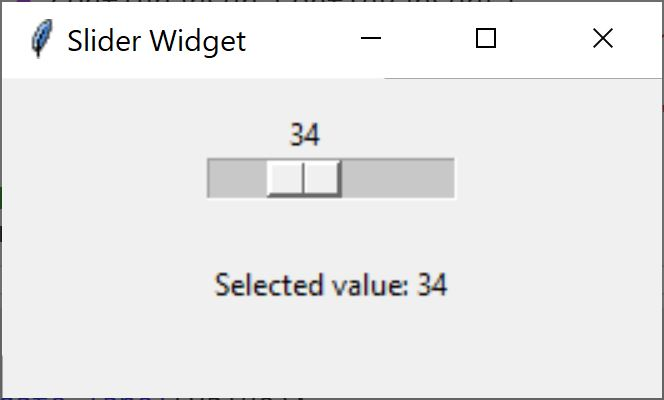
\includegraphics[width=0.4\textwidth]{images/scale_app.JPG}
    \caption{Tkinter Scale App}
    \label{fig:misc-1}
\end{figure}

\newpage
\subsubsection{Tkinter}
\begin{codebox}
\begin{minted}{python}
import tkinter as tk
 
def change_color(event):
    event.widget.configure(bg="red")

root = tk.Tk()
label = tk.Label(root, text="Click me!")
label.bind("<Button-1>", change_color)
label.pack()
 
root.mainloop()
\end{minted}
\end{codebox}
The labels background color will change to red.

\subsubsection{Tkinter - StringVar}
StringVar is a class that provides variable services for Tkinter entry widgets. StringVar is a class in Tkinter used to manipulate string values of Tkinter variables, especially for widgets like Entry and Label, where text can change dynamically.

\newpage
\subsubsection{What is the name of the most general of all Python exceptions?}

BaseException: Exceptions are represented as classes, and they are organized in an inheritance hierarchy. The \texttt{BaseException} class is the root of this hierarchy and serves as the base class for all built-in exceptions in Python.

\subsubsection{Exceptions}
\begin{codebox}
\begin{minted}{python}
def compute(a, b):
    try:
        a / b
    except Exception as exc:
        log(exc)
 
def log(exc):
    logfile = open('logfile.txt')  # Oops, we forgot the 'w' mode.
    print(exc, file=logfile)
    logfile.close()
 
 
compute(0, 0)
\end{minted}
\end{codebox}

\begin{itemize}
\item \textbf{It's an example of implicit exception chaining.} Implicit exception chaining occurs when an exception is caught and a new exception is raised, implicitly attaching the original exception as the cause of the new exception. In this code, the ZeroDivisionError exception is caught in the compute function, and a new exception is raised in the log function. The original exception, ZeroDivisionError, becomes the cause of the new exception.


\item \textbf{This code will raise the ZeroDivisionError exception followed by the FileNotFoundError exception.} In the compute function, the division a / b raises a ZeroDivisionError exception because it attempts to divide by zero. This exception is caught and passed to the log function. However, the log function tries to open the logfile.txt file without the write ('w') mode, leading to a FileNotFoundError exception.

\item The code snippet does \textbf{NOT} demonstrate explicit exception chaining. Explicit exception chaining occurs when one exception is explicitly set as the cause of another exception using the \texttt{raise ... from ...} syntax.
\end{itemize}

\subsubsection{Raising Errors}
In a Python application, you have the following code snippet:

\begin{codebox}
\begin{minted}{python}
try:
    value = int("Hello")
except ValueError as e:
    raise TypeError("Invalid type encountered") from e
\end{minted}
\end{codebox}

\textbf{During the execution, a ValueError is raised in the try block. What happens next?}

A TypeError is raised, and it includes a reference to the original ValueError. Correct as Python's exception chaining mechanism (raise from) attaches the original exception (ValueError) to the new one (TypeError), providing context.

\newpage
\subsubsection{Exceptions}

Implicitly and explicitly chained exceptions refer to how one exception is associated with another in Python:

\begin{itemize}
    \item \textbf{Implicitly Chained Exceptions}:
    \begin{itemize}
        \item When an exception is raised within the handling of another exception, Python automatically sets the \textbf{\texttt{\_\_context\_\_}} attribute of the new exception to the original exception. This creates an implicit chain of exceptions, where the new exception's context is the original exception. This behavior allows you to see the full context in which an exception occurred, helping with debugging and error handling.
    \end{itemize}

    \item \textbf{Explicitly Chained Exceptions}:
    \begin{itemize}
        \item Python also allows you to explicitly chain exceptions using the \textbf{\texttt{raise ... from ...}} syntax. This allows you to raise a new exception while explicitly stating that it was caused by another exception.
        \item This can be useful when you want to raise a higher-level exception that encapsulates the original exception.
    \end{itemize}
\end{itemize}


\begin{itemize}
    \item \textbf{\_\_cause\_\_}: This attribute is for explicitly chained exceptions. It represents the cause of the current exception and is set when one exception is explicitly raised from another using the \texttt{raise ... from ...} syntax.
    
    \item \textbf{\_\_context\_\_}: This attribute is for implicitly chained exceptions. It represents the context in which the current exception occurred. It is automatically set when an exception is raised within the handling of another exception.
    
    \item \textbf{\_\_traceback\_\_}: This attribute is for traceback. It represents the stack trace information associated with the exception. It contains information about the sequence of function calls leading up to the exception.
\end{itemize}

\subsubsection{Explicit exception chaining}
\begin{codebox}
\begin{minted}{python}
class MyCustomException(Exception):
    pass
 
 
def compute(val1, val2):
    try:
        result = val1 / val2
    except ZeroDivisionError as e:
        raise MyCustomException from e
    return result
 
 
compute(1, 0)
\end{minted}
\end{codebox}
In this case, the \texttt{raise MyCustomException from e} statement explicitly raises \texttt{MyCustomException} and links it to the \texttt{ZeroDivisionError (e)} as the cause. This is an example of explicit exception chaining, where the developer deliberately associates the new exception with the original one.

\newpage
\subsubsection{User-defined Exceptions}
In Python, when defining a user-defined exception, it is recommended to derive it from the built-in \texttt{Exception} class or one of its subclasses. The \texttt{Exception} class is the base class for all built-in exceptions in Python.

By deriving a user-defined exception from the \texttt{Exception} class, you inherit the behavior and characteristics of the \texttt{Exception} class. This includes features such as message handling, traceback information, and compatibility with exception handling mechanisms in Python.

\subsubsection{What is the expected output of the following code?}
\begin{codebox}
\begin{minted}{python}
class NewError(Exception):
    def __init__(self, name, color):
        self.data = (name, color)
 
 
try:
    raise NewError('New warning!', 'Red alert!')
except NewError as e:
    # print(e.args) # ('New warning!', 'Red alert!')
    print(' '.join(e.args)) # New warning! Red alert!
\end{minted}
\end{codebox}

The \texttt{args} attribute of the \texttt{NewError} exception is initialized with the tuple \texttt{('New warning!', 'Red alert!')} in the \texttt{\_\_init\_\_} method. In the \texttt{except} block, we print the joined elements of this tuple, resulting in the output "New warning! Red alert!".

\subsubsection{\texttt{json.dumps()}}
The \texttt{json.dumps()} function is used to convert Python objects to JSON-formatted strings. Not all Python objects are JSON serializable. When json.dumps() encounters an object that is not serializable, it raises a \textbf{TypeError} exception.

\begin{codebox}
\begin{minted}{python}
import json

# Example Python dictionary
data = {
    "name": "John",
    "age": 30,
    "city": "New York"
}

# Serialize the dictionary to a JSON formatted string
json_string = json.dumps(data)

# Output the JSON formatted string
print(json_string)
\end{minted}
\end{codebox}

\newpage
\subsubsection{Suppose you have the following \texttt{Vector} class and \texttt{ecnode\_vector()} function. What is the result of the following code?}
\begin{codebox}
\begin{minted}{python}
import json

class Vector:
    def __init__(self, *components):
        print(components)   # Output: (1, 2, 3)
        self.components = components
 
    def __repr__(self):
        return f'Vector{self.components}'
 
    def __str__(self):
        return f'{self.components}'
 
 
def encode_vector(v):
    if isinstance(v, Vector):
        print(v.__dict__)   # Output: {'components': (1, 2, 3)}
        return v.__dict__
    else:
        raise TypeError(
            f'Object of type {v.__class__.__name__} is not JSON serializable'
        )

v1 = Vector(1, 2, 3)
print(json.dumps(v1, default=encode_vector))   
# Output: {"components": [1, 2, 3]}
\end{minted}
\end{codebox}

The \texttt{json.dumps()} function is used to serialize Python objects to a JSON formatted string. It takes a Python object (such as a dictionary, list, tuple, etc.) as input and returns a string representing that object in JSON format. The \texttt{default} parameter is an optional parameter that allows you to specify a function that will be called for objects that are not serializable by default. This function should return a serializable version of the object, or raise a \texttt{TypeError} if it cannot do so.

\newpage
\subsubsection{Coding}

\begin{codebox}
\begin{minted}{python}
class IntegerList(list):
 
    @staticmethod
    def check_type(value):
        if type(value) is not int:
            raise ValueError('The value must be of type int.')
 
    def __setitem__(self, index, value):
        IntegerList.check_type(value)
        list.__setitem__(self, index, value)
 
    def append(self, value):
        IntegerList.check_type(value)
        list.append(self, value)        
 
    def extend(self, iterable):
        for element in iterable:
            IntegerList.check_type(element)
        list.extend(self, iterable)
\end{minted}
\end{codebox}

\textbf{Which of the following operations will run without errors?}

\begin{codebox}
\begin{minted}{python}
integers = IntegerList([1, 2, 3])
integers[1] = 0
\end{minted}
\end{codebox}

\begin{codebox}
\begin{minted}{python}
integers = IntegerList([1, 2, 3])
integers.extend([4, 5])
\end{minted}
\end{codebox}

\newpage
\subsubsection{Asterisks in function definition}
\textbf{What do the asterisks in the function definition mean?}\\
They denote parameters that should be unpacked before use. In Python function definitions, the asterisks (\texttt{*} and \texttt{**}) have special meanings when used in the parameter list. They are used to handle variable-length arguments and to unpack iterables or dictionaries.

\begin{itemize}
    \item \textbf{*args}: When an asterisk is prefixed before a parameter name in a function definition (e.g., *args), it allows the function to accept any number of positional arguments. These arguments are packed into a tuple within the function, allowing you to pass a variable number of arguments to the function.
    \item \textbf{**kwargs}: When two asterisks are prefixed before a parameter name in a function definition (e.g., **kwargs), it allows the function to accept any number of keyword arguments. These arguments are packed into a dictionary within the function, allowing you to pass a variable number of keyword arguments to the function.
\end{itemize}

\subsubsection{Function calls}
\begin{codebox}
\begin{minted}{python}
def process_data(*args, **kwargs):
    if "mode" in kwargs:
        mode = kwargs['mode']
        if mode == 'sum':
            result = sum(args)
        elif mode == 'product':
            result = 1
            for arg in args:
                result *= arg
        else:
            result = None
    else:
        result = None
 
    return result
\end{minted}
\end{codebox}
\textbf{Which of the following function calls will correctly compute the product of the given numbers?}

\texttt{process\_data(2, 4, 6, mode='product')}: This function call correctly passes the numbers 2, 4, 6 as non-keyword arguments and specifies the keyword argument 'mode' with the value 'product'. It will correctly compute the product of the numbers.

\newpage
\subsubsection{Dictionaries}
\begin{codebox}
\begin{minted}{python}
def merge_dicts(*dicts, **kwargs):
    merged_dict = {}
    for dictionary in dicts:
        print(dictionary)
        merged_dict.update(dictionary)
    merged_dict.update(kwargs)
    return merged_dict


dict1 = {"name": "John", "age": 30}
dict2 = {"city": "New York", "country": "USA"}
dict3 = {"occupation": "Engineer"}
 
merge_dicts(dict1, dict2, dict3, skill="Python", experience=5)
\end{minted}
\end{codebox}

\subsubsection{Context manager}
In Python, a context manager is an object that is used to manage resources and define setup and teardown actions that need to be performed around a block of code. It allows you to allocate and release resources precisely when they are needed, such as opening and closing files, acquiring and releasing locks, and connecting to and disconnecting from databases.

\begin{codebox}
\begin{minted}{python}
# Using a context manager to open and close a file
with open('example.txt', 'r') as file:
    data = file.read()
    # Perform operations with the file

# At this point, the file is automatically closed
\end{minted}
\end{codebox}
In this example, the \texttt{open()} function returns a file object, which acts as a context manager. When the \texttt{with} statement is executed, it calls the \texttt{\_\_enter\_\_()} method of the file object to open the file. After the code block executes, the \texttt{\_\_exit\_\_()} method is called to close the file, ensuring that the file is properly closed even if an exception occurs within the block.\\

It is not necessary to explicitly call the close() method when using a context manager since it automatically takes care of closing the file.